% ChronoLeak presentation: Part I (AES Under the Microscope) and Part II (ChronoLeak plan)
% Build with scripts/docs.sh (or: tectonic -X compile slides.tex, run inside presentation/beamer/)
\documentclass[aspectratio=169,11pt]{beamer}
\usepackage{fontspec}
\setsansfont{texgyreheros}[Extension=.otf, UprightFont=*-regular, BoldFont=*-bold, ItalicFont=*-italic, BoldItalicFont=*-bolditalic]
\setmonofont{texgyrecursor}[Extension=.otf, UprightFont=*-regular, BoldFont=*-bold, Scale=0.95]
\usepackage{booktabs,array,tikz,amsmath}
\usetikzlibrary{arrows.meta,positioning,fit,calc,backgrounds}
\graphicspath{{../../results/full-20261117-0301/figures/}{../../presentation/img/}{../../report/latex/}}

% ---- look ----------------------------------------------------------------------------
\definecolor{ink}{HTML}{111111}
\definecolor{accent}{HTML}{B8302F}
\definecolor{navy}{HTML}{1F3A5F}
\definecolor{soft}{HTML}{F3F2EF}
\setbeamercolor{normal text}{fg=ink,bg=white}
\setbeamercolor{frametitle}{fg=navy,bg=white}
\setbeamercolor{title}{fg=white}
\setbeamercolor{structure}{fg=navy}
\setbeamercolor{alerted text}{fg=accent}
\setbeamercolor{block title}{fg=white,bg=navy}
\setbeamercolor{block body}{bg=soft}
\setbeamertemplate{navigation symbols}{}
\setbeamertemplate{itemize items}{\color{accent}$\bullet$}
\setbeamertemplate{itemize subitem}{\color{navy}--}
\setbeamerfont{frametitle}{size=\Large,series=\bfseries}
\setbeamertemplate{frametitle}{\vspace{0.35cm}\insertframetitle\par\vspace{-0.1cm}{\color{accent}\rule{1.4cm}{1.5pt}}}
\setbeamertemplate{footline}{%
  \hbox to \paperwidth{\hspace{0.5cm}{\tiny\color{gray}ChronoLeak \textbullet{} Bibek Chaudhary (23ECB0F33) \textbullet{} Cryptography and Network Security}\hfill{\tiny\color{gray}\insertframenumber/\inserttotalframenumber}\hspace{0.5cm}}\vspace{0.25cm}}
\newcommand{\code}[1]{\texttt{#1}}
\newcommand{\partslide}[2]{{\setbeamercolor{background canvas}{bg=navy}\setbeamertemplate{footline}{}
\begin{frame}[plain]\color{white}\vfill{\large\color{white!70}#1}\par\vspace{0.2cm}{\Huge\bfseries #2}\par\vfill\end{frame}}}
\tikzset{
  box/.style={draw=black!70, rounded corners=3pt, align=center, font=\footnotesize, inner sep=4pt, minimum height=8mm, line width=0.5pt},
  impl/.style={box, fill=orange!14}, sw/.style={box, fill=blue!8}, res/.style={box, fill=green!12},
  note/.style={draw=black!50, fill=gray!10, align=center, font=\footnotesize, inner sep=4pt},
  arr/.style={-{Latex[length=2mm]}, line width=0.7pt, draw=black!80}, darr/.style={arr, dashed},
}

\begin{document}

% ---------------------------------------------------------------- title
{\setbeamercolor{background canvas}{bg=ink}\setbeamertemplate{footline}{}
\begin{frame}[plain]
\color{white}
\vspace{0.6cm}
{\Huge\bfseries ChronoLeak}\par\vspace{0.15cm}
{\Large Timing side-channel leakage in cryptographic implementations}\par\vspace{0.5cm}
{\normalsize\color{white!85}Part I: \textbf{AES Under the Microscope}, an experimental study of AES-128 on Apple M4\\
Part II: \textbf{ChronoLeak}, compiler-induced timing leakage in Rust cryptography (plan)}\par
\vspace{0.7cm}
{\small Bibek Chaudhary (23ECB0F33)\\ Course: Cryptography and Network Security \quad Guide: Prof.\ Sourabh Solanki\\
Department of ECE, National Institute of Technology Warangal \quad November 2026}
\vfill
\end{frame}}

\begin{frame}{Same cipher. Same output. Different timing?}
\begin{itemize}
  \item AES has survived 25 years of cryptanalysis; attackers break the \alert{implementation}, not the maths
  \item Kocher (1996): running time leaks keys \quad Bernstein; Osvik, Shamir \& Tromer (2005--06): AES table lookups leak through the cache
  \item Defence: \alert{constant-time} code, with no secret-dependent branches or memory addresses
  \item But the code that runs is what the \alert{compiler} produced, on a processor with its own \alert{predictors}
\end{itemize}
\vspace{0.3cm}
\begin{block}{Question of the project}
When does code written to be constant-time actually run in constant time, and when can a difference be measured?
\end{block}
\end{frame}

\begin{frame}{Two parts}
\centering
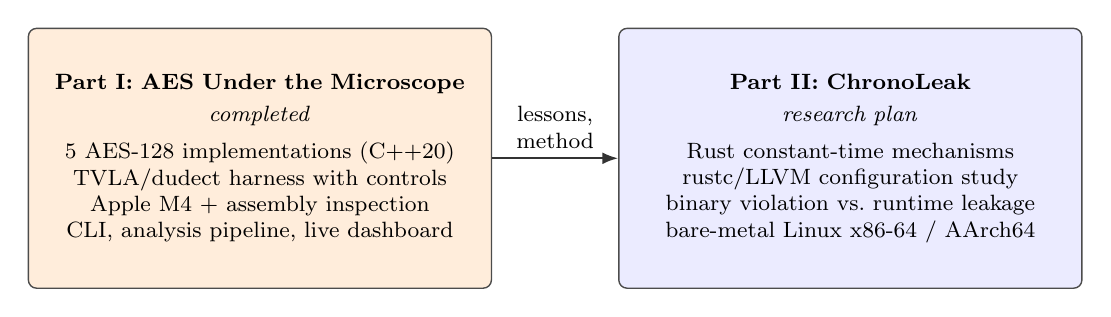
\begin{tikzpicture}
  \node[impl, text width=5.6cm, minimum height=3.3cm] (p1) {\textbf{Part I: AES Under the Microscope}\\[2pt] \emph{completed}\\[4pt] 5 AES-128 implementations (C++20)\\ TVLA/dudect harness with controls\\ Apple M4 + assembly inspection\\ CLI, analysis pipeline, live dashboard};
  \node[sw, right=1.6cm of p1, text width=5.6cm, minimum height=3.3cm] (p2) {\textbf{Part II: ChronoLeak}\\[2pt] \emph{research plan}\\[4pt] Rust constant-time mechanisms\\ rustc/LLVM configuration study\\ binary violation vs.\ runtime leakage\\ bare-metal Linux x86-64 / AArch64};
  \draw[arr] (p1) -- node[above, font=\footnotesize, align=center]{lessons,\\ method} (p2);
\end{tikzpicture}
\vspace{0.4cm}

{\small Outline: background \textbullet{} literature review \textbullet{} Part I system \textbullet{} live demo \textbullet{} results \textbullet{} Part II plan \textbullet{} conclusion}
\end{frame}

% ---------------------------------------------------------------- background
\begin{frame}{AES-128 in one picture}
\begin{columns}[T]
\begin{column}{0.55\textwidth}
\begin{itemize}
  \item 128-bit block $\rightarrow$ $4\times4$ byte \alert{state}
  \item 128-bit key $\rightarrow$ \alert{11 round keys} (RotWord, SubWord, Rcon)
  \item AddRoundKey, then 10 rounds:\\ SubBytes $\rightarrow$ ShiftRows $\rightarrow$ MixColumns $\rightarrow$ AddRoundKey
  \item Round 10 drops MixColumns: it is linear and adds nothing there
  \item Our code reproduces FIPS-197 C.1:\\ {\footnotesize\code{69c4e0d86a7b0430d8cdb78070b4c55a}}
\end{itemize}
\end{column}
\begin{column}{0.42\textwidth}
\begin{block}{The maths: GF($2^8$)}
\small
Bytes are polynomials mod $m(x) = x^8+x^4+x^3+x+1$\\[3pt]
Addition = XOR, $\mathrm{xtime}(a) = (a\ll1)\oplus(\texttt{0x1B}\cdot a_7)$\\[3pt]
S-box: $S(a) = A(a^{-1})\oplus\texttt{0x63}$, \quad $a^{-1} = a^{254}$\\[3pt]
MixColumns: MDS matrix, full diffusion after 2 rounds
\end{block}
\small The constant-time version \alert{computes} $a^{254}$ instead of looking it up.
\end{column}
\end{columns}
\end{frame}

\begin{frame}{Timing side channels and how to test for them}
\begin{columns}[T]
\begin{column}{0.5\textwidth}
\textbf{Two leaks}
\begin{itemize}
  \item \alert{Secret branch}: \code{if (secret) work();}
  \item \alert{Secret address}: \code{T[secret]} touches a cache line chosen by the secret; T-table AES does 160 per block
\end{itemize}
\textbf{Defences}: no tables (bit-slicing, vector permute, computed S-box) or hardware AES
\end{column}
\begin{column}{0.47\textwidth}
\textbf{Fixed-vs-random test} (TVLA 2011, dudect 2017)
\begin{itemize}
  \item coin flip: \alert{fixed} or \alert{random} input
  \item Welch: $t = \dfrac{\bar x_F - \bar x_R}{\sqrt{s_F^2/n_F + s_R^2/n_R}}$
  \item $\lvert t\rvert > 4.5$ $\Rightarrow$ leakage detected
  \item says \emph{whether}, not \emph{how}; non-detection is not proof
\end{itemize}
\end{column}
\end{columns}
\end{frame}

% ---------------------------------------------------------------- literature
\begin{frame}{Literature review}
\scriptsize
\renewcommand{\arraystretch}{1.0}
\begin{tabular}{@{}>{\raggedright\arraybackslash}p{0.33\textwidth}>{\raggedright\arraybackslash}p{0.32\textwidth}>{\raggedright\arraybackslash}p{0.27\textwidth}@{}}
\toprule
Work & Contribution & Open point for us \\
\midrule
Kocher '96; Bernstein '05; Osvik '06 & Timing and cache attacks on AES & Behaviour on Apple M4 \\
TVLA '11; dudect '17; Welch '47 & Fixed-vs-random leakage test & Controls; bounds on non-detection \\
Käsper--Schwabe '09; Hamburg '09 & Constant-time AES & Empirical check on a real CPU \\
GoFetch '24; SLAP, FLOP '25 & Apple prefetcher/predictors leak & Effect on leakage tests unknown \\
\alert{Breaking Bad} (ASIA CCS '25) & Compilers break CT code (8 libs, 6 archs) & No Rust targets \\
\alert{Fun with Flags} (PriSC '26); DOCC (FC '25) & Passes behind violations & C only \\
RoboCop (PLDI '25); LLVM \code{ct.select} & Compiler defences & Not exposed in Rust \\
ctgrind; MicroWalk; Pitchfork; AutoBench-CT & Analysis tools, benchmark & Rarely tied to timing \\
\code{subtle}; \code{black\_box}; RUSTSEC-2025-0144 & Rust CT mechanisms; ML-DSA CVE & Never measured \\
\bottomrule
\end{tabular}
\end{frame}

\partslide{Part I}{AES Under the Microscope}

\begin{frame}{Five implementations, leaky $\rightarrow$ hardware}
\centering\small
\renewcommand{\arraystretch}{1.15}
\begin{tabular}{@{}llcr@{}}
\toprule
& Strategy & Secret-indexed loads & Latency \\
\midrule
\code{ref} & textbook, 256 B S-box & 32 & 169 ns \\
\code{ttable} & $4\times1$ KB T-tables & 32 & 36 ns \\
\code{ct} & computed S-box, no tables & \alert{0} & 2,559 ns \\
\code{armv8} & \code{AESE}/\code{AESMC} hardware & \alert{0} & \alert{7.2 ns} \\
\code{openssl} & OpenSSL 3.6.1 EVP, default path & 0 & 8.0 ns \\
\bottomrule
\end{tabular}

\vspace{0.4cm}
\raggedright
\begin{itemize}
  \item All five agree on \alert{100,000 random inputs}; 43 self-test checks; ASan/UBSan clean
  \item \textbf{Positive control}: an \emph{intentionally injected} secret branch (not a weakness of AES) and its branch-free twin
\end{itemize}
\end{frame}

\begin{frame}{What we built}
\begin{columns}[c]
\begin{column}{0.52\textwidth}
\centering
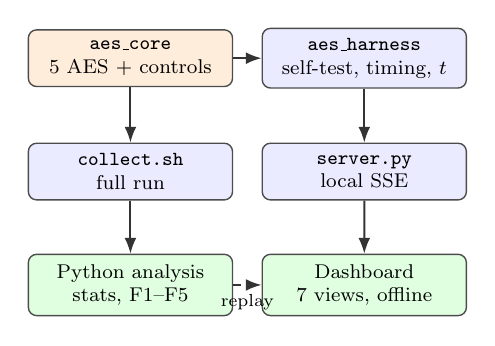
\begin{tikzpicture}[scale=0.9, transform shape]
  \node[impl, text width=2.6cm] (core) at (0,0) {\code{aes\_core}\\ 5 AES + controls};
  \node[sw, text width=2.6cm] (harn) at (3.3,0) {\code{aes\_harness}\\ self-test, timing, $t$};
  \draw[arr] (core) -- (harn);
  \node[sw, text width=2.6cm] (col) at (0,-1.6) {\code{collect.sh}\\ full run};
  \node[sw, text width=2.6cm] (srv) at (3.3,-1.6) {\code{server.py}\\ local SSE};
  \node[res, text width=2.6cm] (ana) at (0,-3.2) {Python analysis\\ stats, F1--F5};
  \node[res, text width=2.6cm] (web) at (3.3,-3.2) {Dashboard\\ 7 views, offline};
  \draw[arr] (core) -- (col); \draw[arr] (harn) -- (srv); \draw[arr] (col) -- (ana); \draw[arr] (srv) -- (web);
  \draw[darr] (ana) -- node[below, font=\scriptsize]{replay} (web);
\end{tikzpicture}
\end{column}
\begin{column}{0.46\textwidth}
\small
\begin{itemize}
  \item One C++20 binary, \alert{10 commands}; refuses to time anything until the self-test passes
  \item Harness: coin flip $\rightarrow$ identical input prep $\rightarrow$ (evict 4 MB) $\rightarrow$ time $B$ encryptions
  \item Timer: \code{mach\_absolute\_time}, 24 MHz = 41.67 ns/tick
  \item Python recomputes every statistic from raw samples
  \item 3 ctest suites + 110-check end-to-end suite
\end{itemize}
\end{column}
\end{columns}
\end{frame}

\begin{frame}{The dashboard}
\centering
\begin{tabular}{@{}cc@{}}
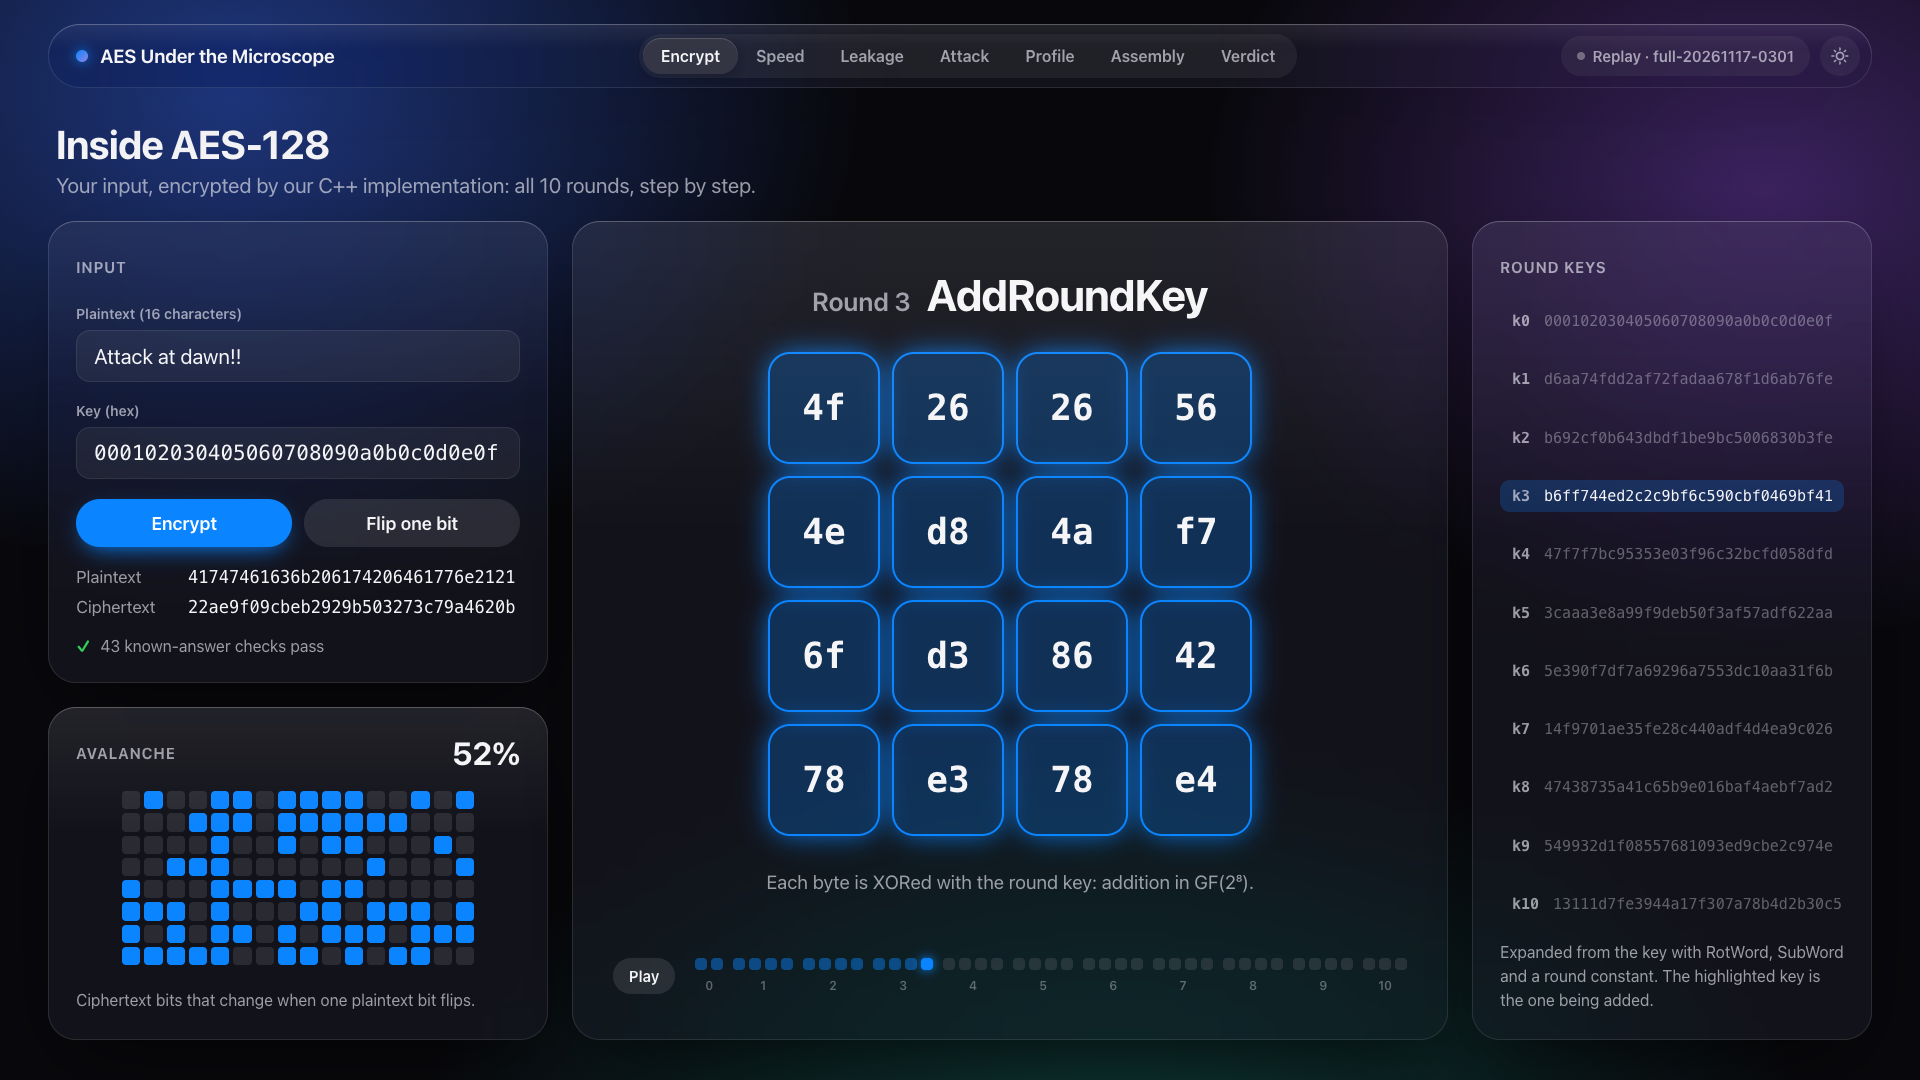
\includegraphics[width=0.36\textwidth]{dash_explorer.png} & 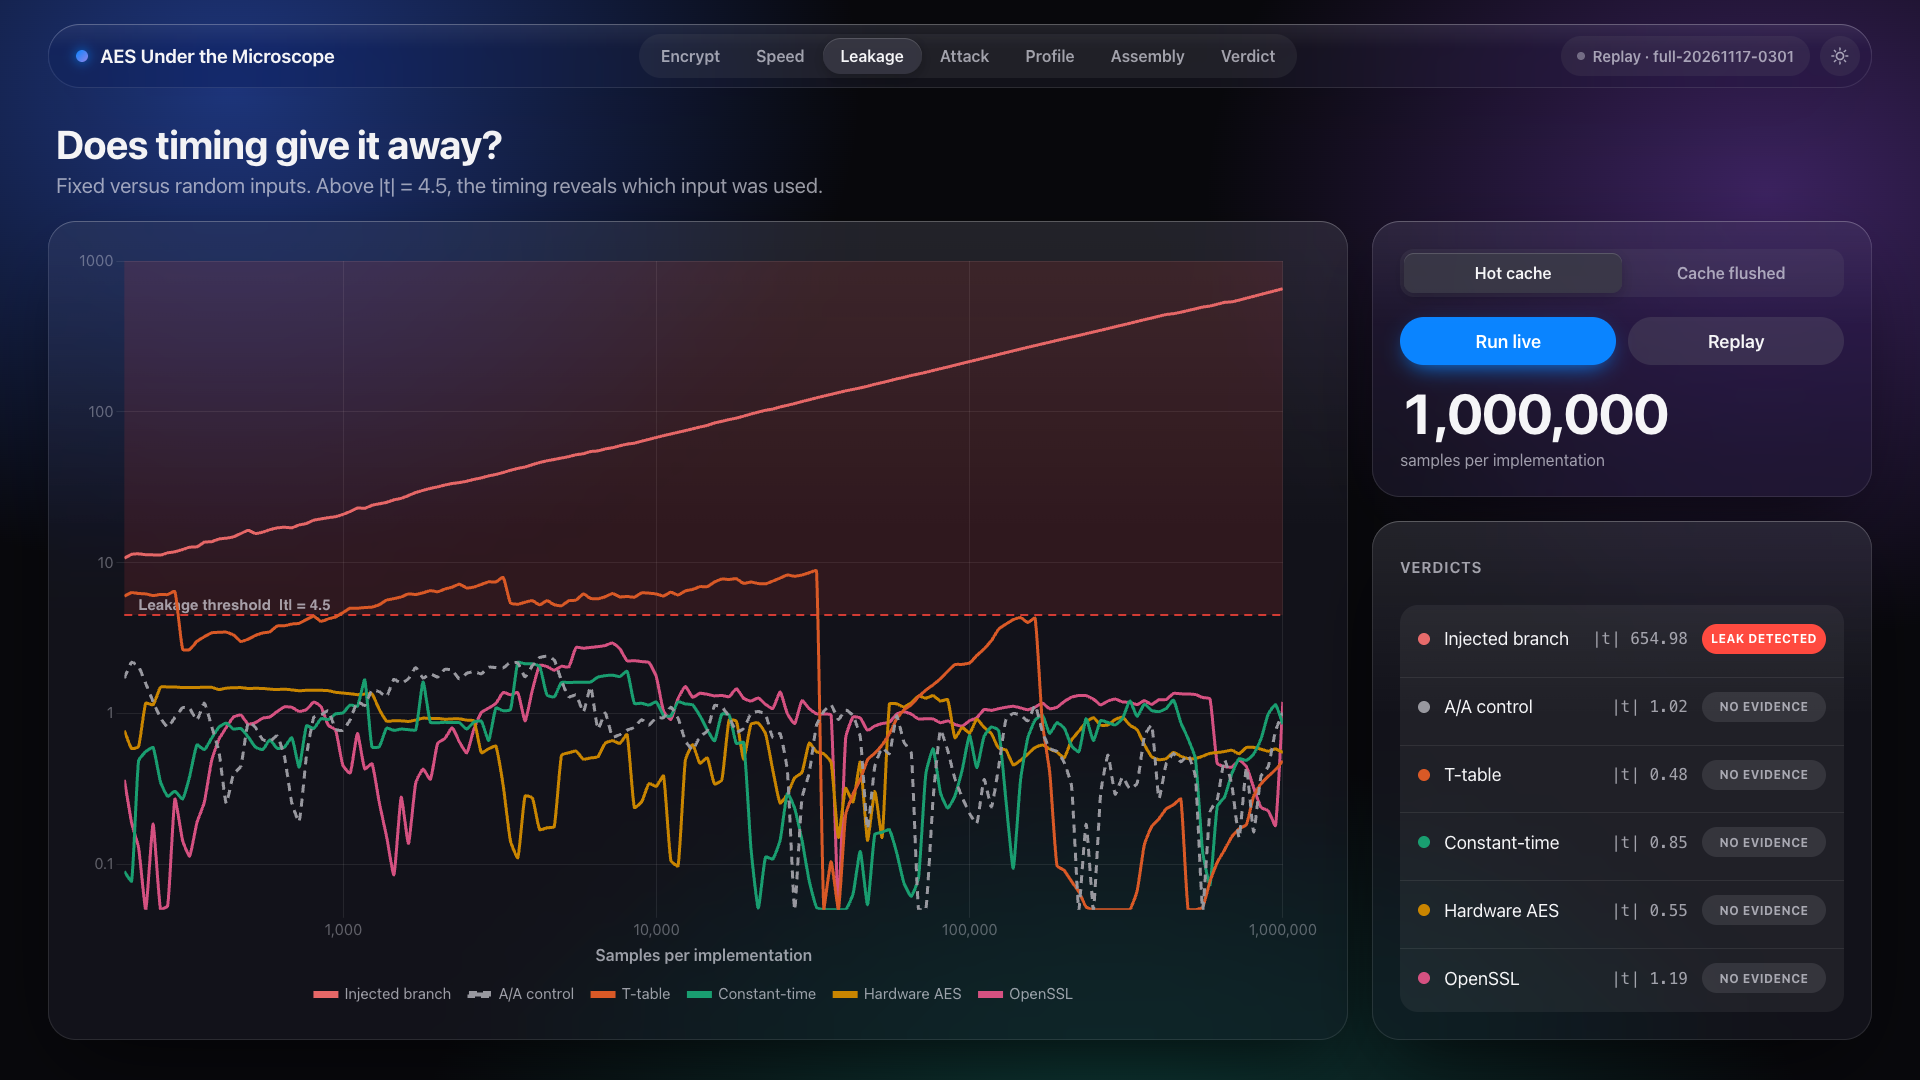
\includegraphics[width=0.36\textwidth]{dash_race.png}\\[-1pt]
{\scriptsize Encrypt: rounds, round keys, avalanche} & {\scriptsize Leakage race: $\lvert t\rvert$ vs.\ samples}\\[4pt]
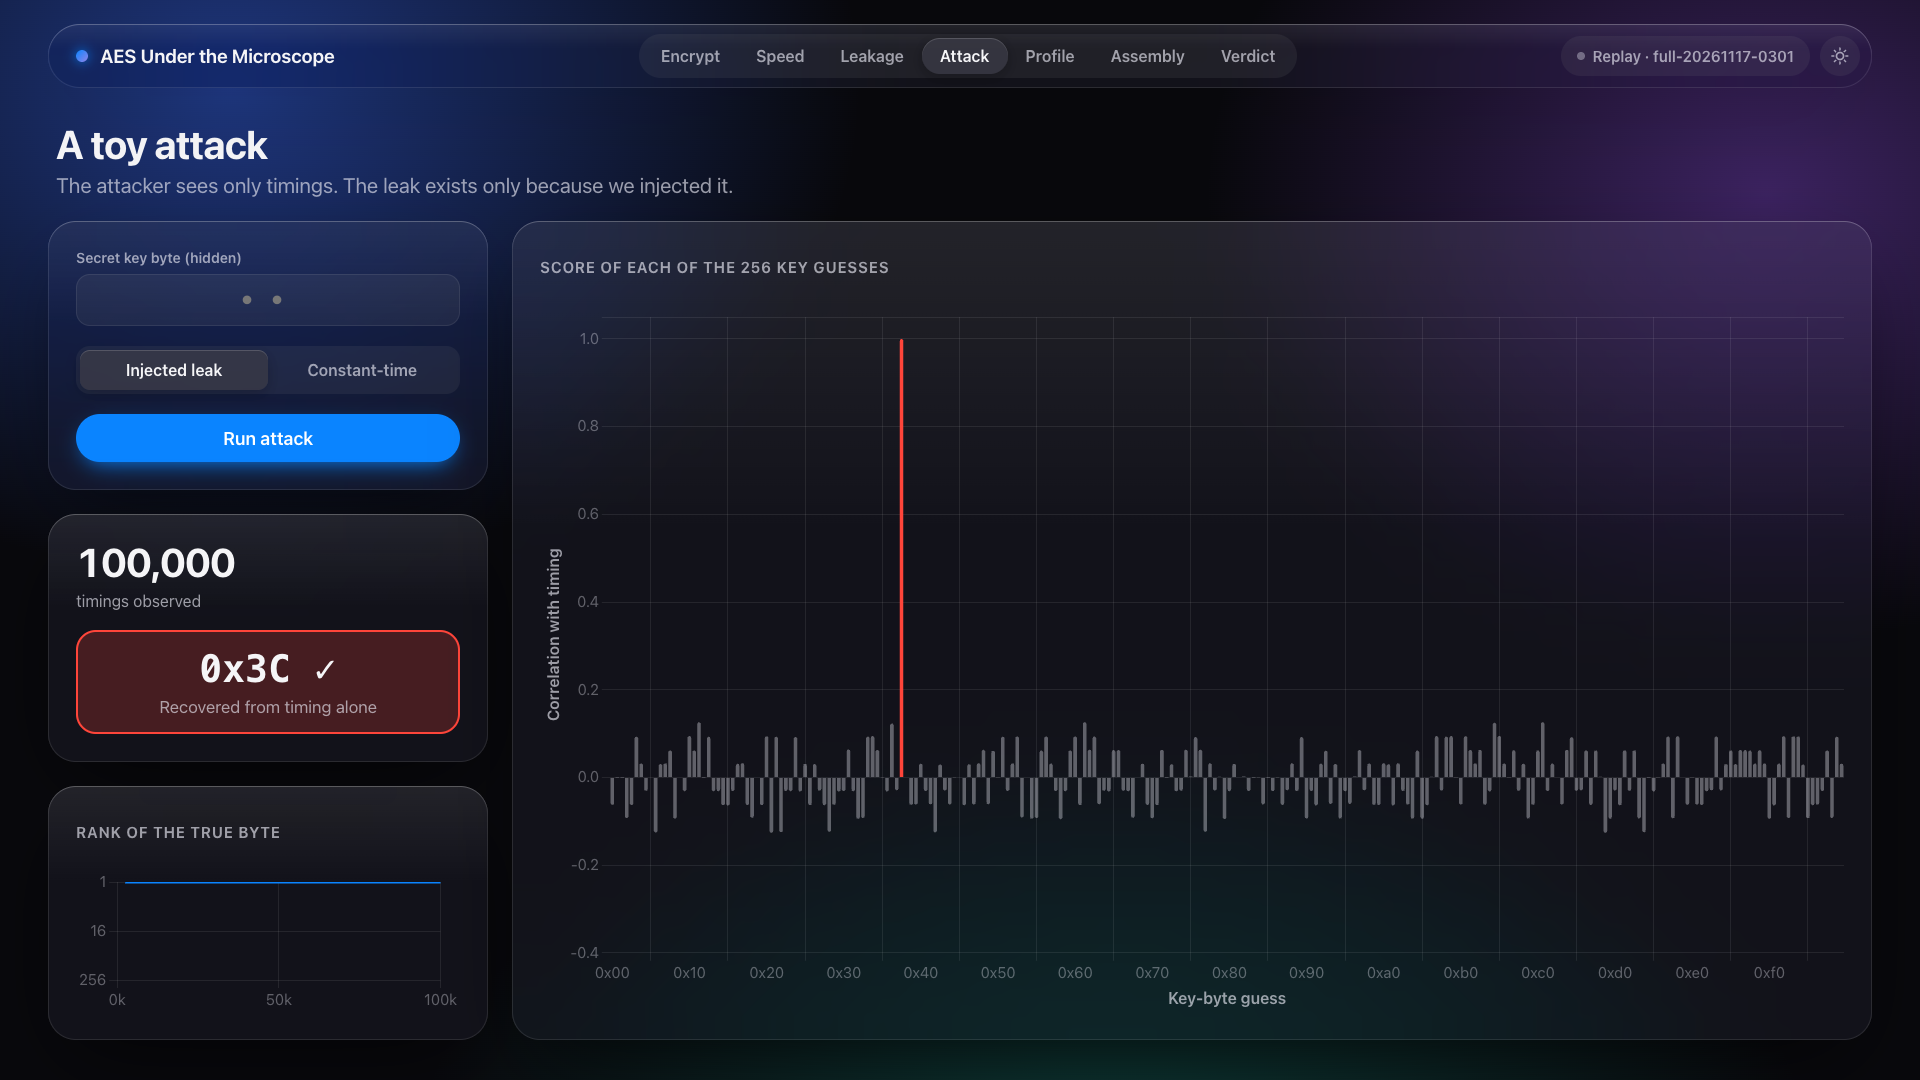
\includegraphics[width=0.36\textwidth]{dash_heist.png} & 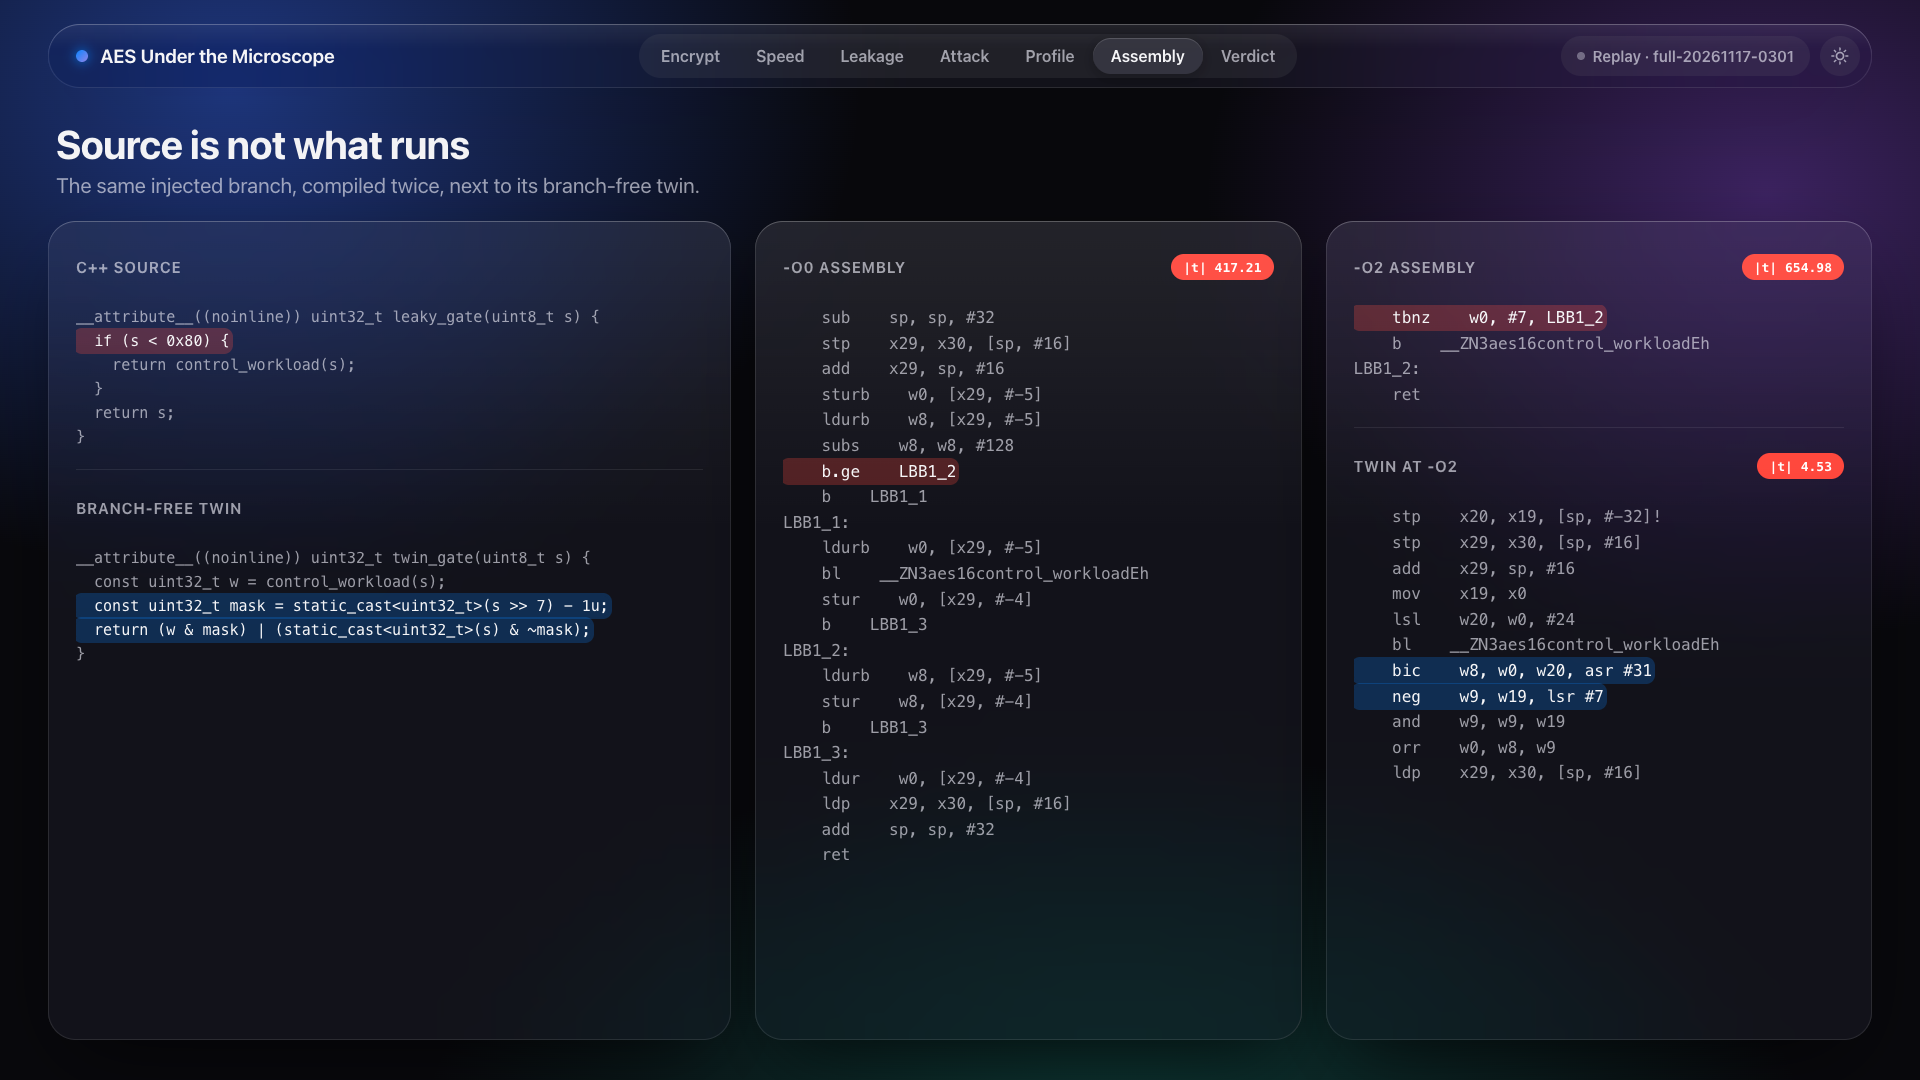
\includegraphics[width=0.36\textwidth]{dash_compiler.png}\\[-1pt]
{\scriptsize Toy attack: byte recovered from timing (injected leak only)} & {\scriptsize Assembly: branch survives as \code{tbnz}}
\end{tabular}
\end{frame}

\begin{frame}{Methodology}
\begin{columns}[T]
\begin{column}{0.5\textwidth}
\begin{itemize}
  \item $10^6$ samples per test, classes interleaved at random
  \item \alert{Hot} cache, and \alert{evicted}: 4 MB read before every sample, $B = 1$
  \item Primary statistic fixed in advance: Welch $\lvert t\rvert > 4.5$
  \item Also: cropped $t$, Mann--Whitney, KS, Holm correction, minimum detectable difference
\end{itemize}
\end{column}
\begin{column}{0.47\textwidth}
\textbf{Hypotheses, written before data}
\small
\begin{description}[H0]
  \item[H0] A/A negative control stays below 4.5
  \item[H1] Injected branch is detected
  \item[H2] T-table leaks under eviction
  \item[H3] \code{ct} and \code{armv8} show nothing
  \item[H4] OpenSSL depends on its code path
\end{description}
\end{column}
\end{columns}
\end{frame}

{\setbeamercolor{background canvas}{bg=soft}\setbeamertemplate{footline}{}
\begin{frame}[plain]
\centering\vfill
{\Huge\bfseries Live demo}\par\vspace{0.4cm}
{\large Encrypt $\rightarrow$ Speed $\rightarrow$ \alert{Leakage race} $\rightarrow$ \alert{Attack} $\rightarrow$ Assembly $\rightarrow$ Verdict}\par\vspace{0.3cm}
{\small\code{scripts/demo.sh} \textbullet{} fully offline \textbullet{} every number from the C++ binary}
\vfill
\end{frame}}

\begin{frame}{Results: leakage}
\begin{columns}[c]
\begin{column}{0.40\textwidth}
\small
\renewcommand{\arraystretch}{1.1}
\begin{tabular}{@{}lr@{}}
\toprule
Test & $\lvert t\rvert$ \\
\midrule
positive control & \alert{655} \\
A/A control & 1.02 \\
\alert{ttable, evicted} & \alert{18.8} \\
ttable, hot & 0.48 \\
ct / armv8 & $\le$ 1.10 \\
OpenSSL default & $\le$ 1.79 \\
OpenSSL armcap=0 (hot) & 19.8$^*$ \\
\bottomrule
\end{tabular}

\vspace{0.2cm}
{\scriptsize $^*$hot-regime confound, see limitations\\ T-table: +3.1 ns on 81 ns}
\end{column}
\begin{column}{0.56\textwidth}
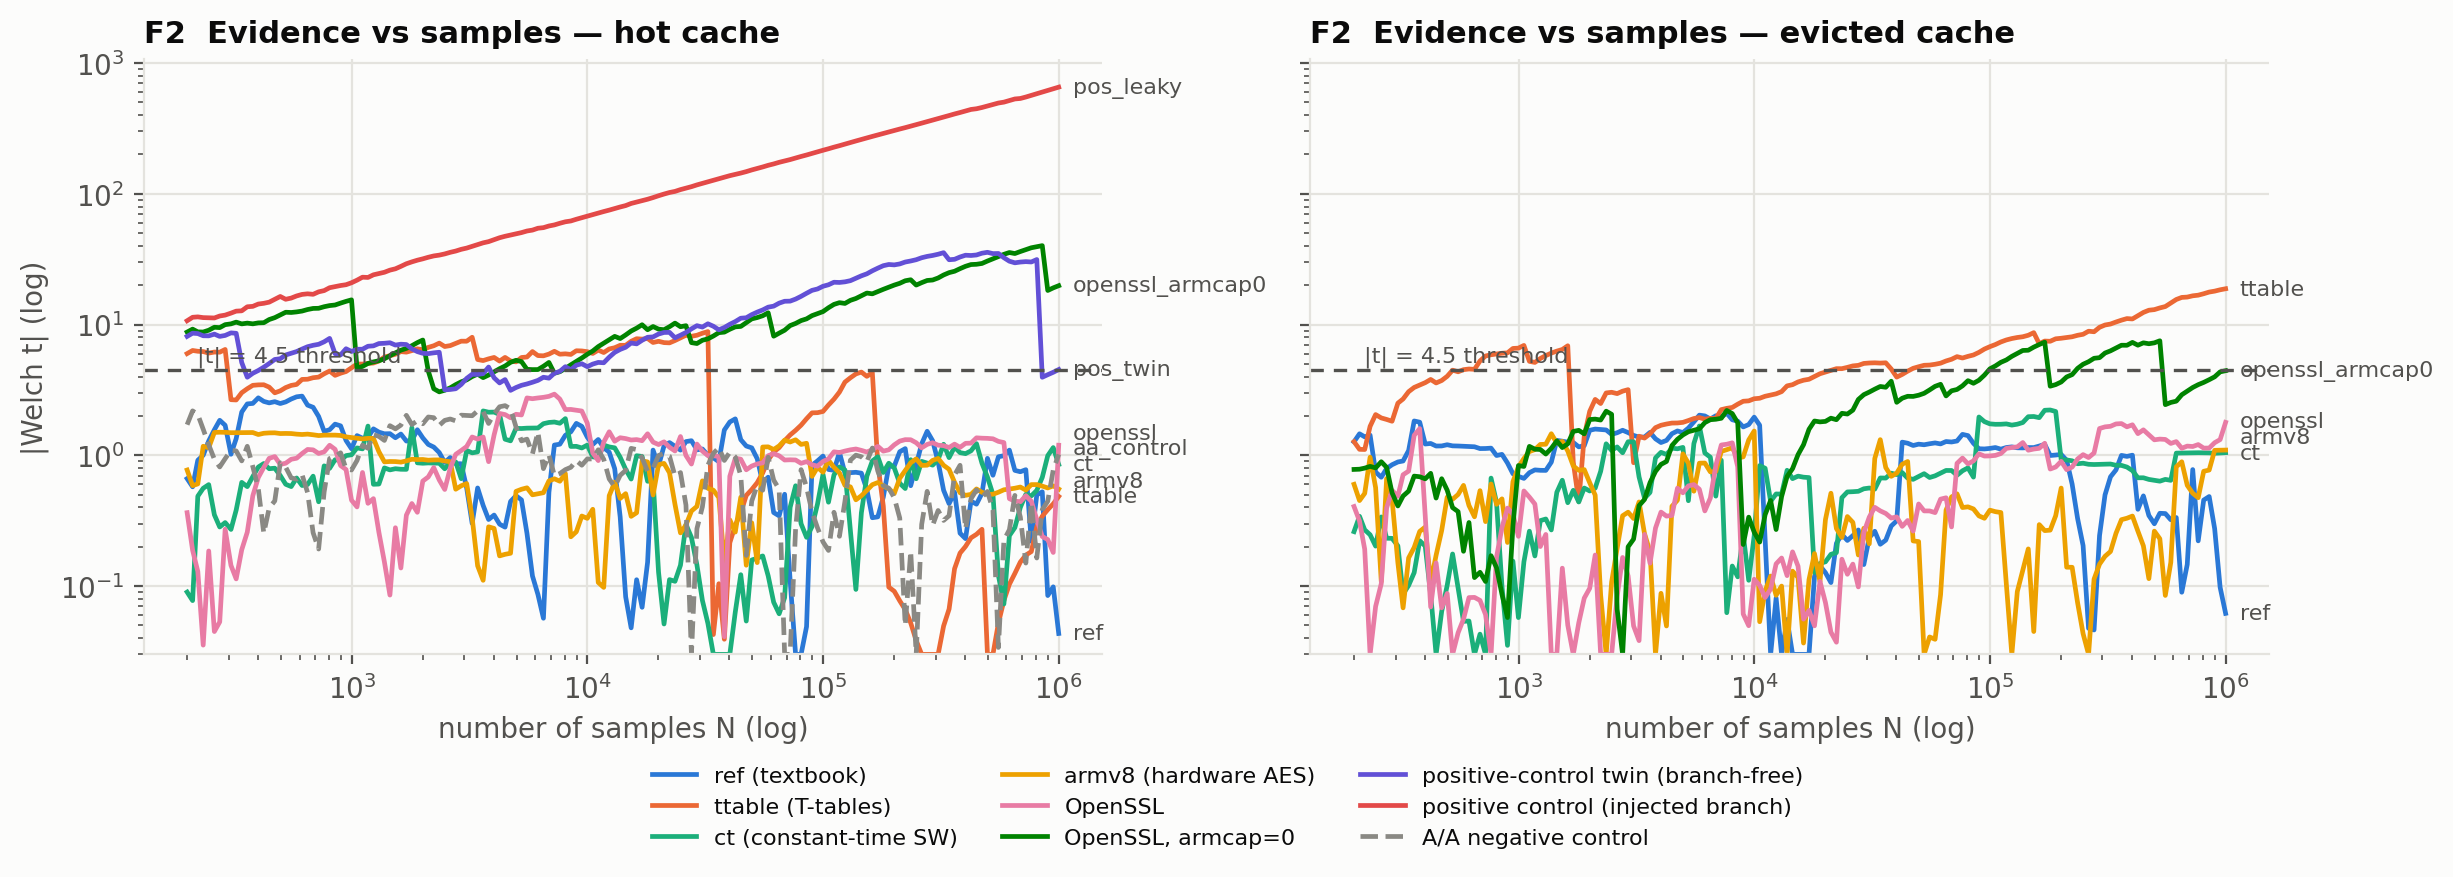
\includegraphics[width=\textwidth]{F2_t_vs_n.png}
\end{column}
\end{columns}
\end{frame}

\begin{frame}{Results: performance and compiler}
\begin{columns}[c]
\begin{column}{0.5\textwidth}
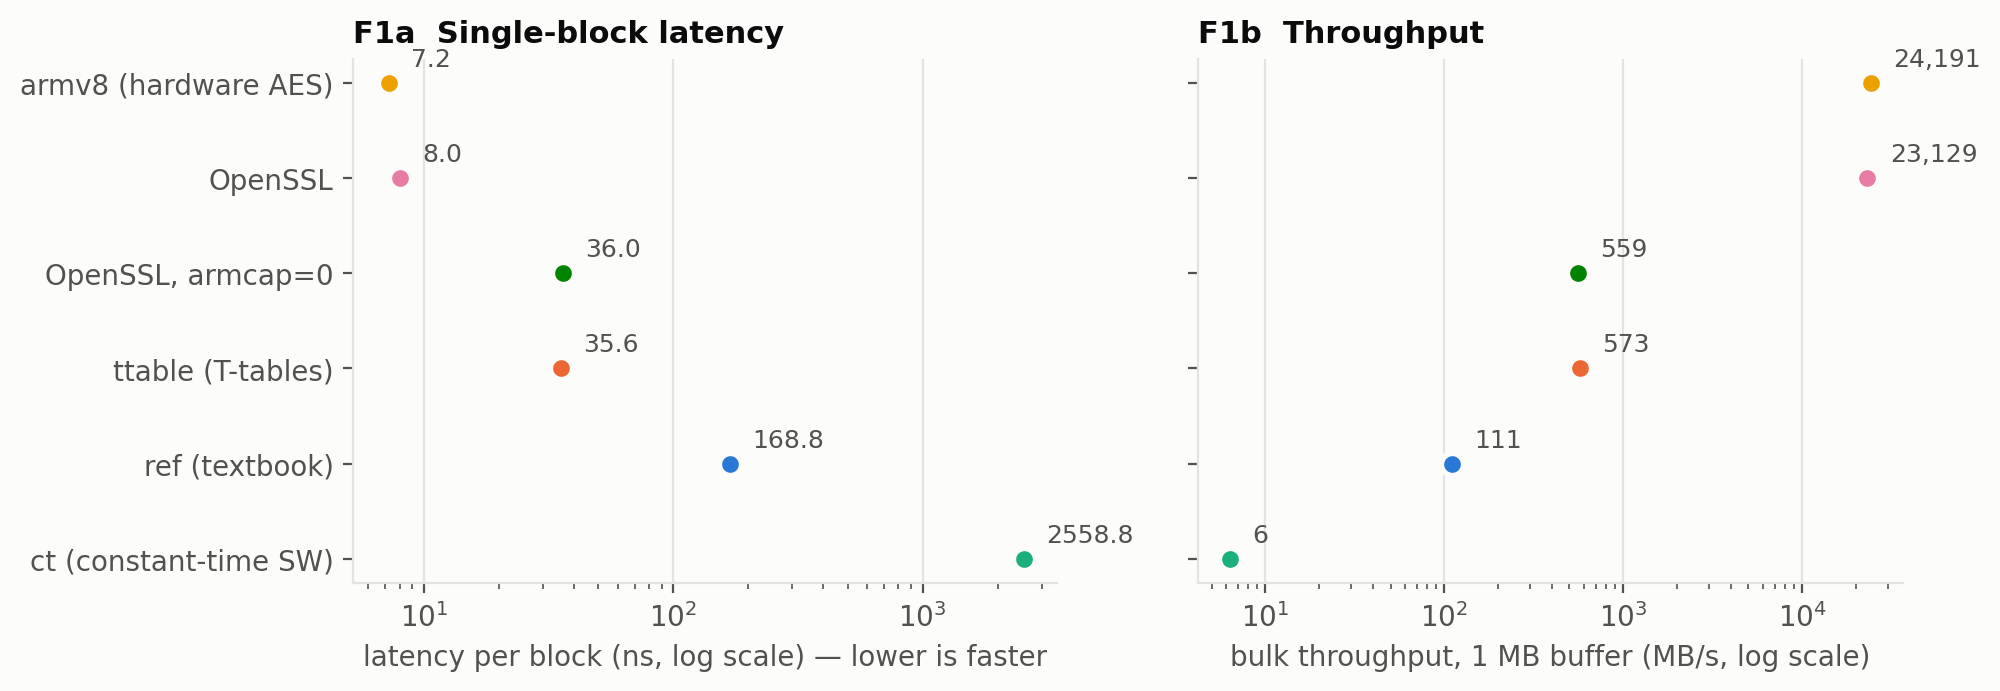
\includegraphics[width=\textwidth]{F1_performance.png}\\
{\scriptsize Hardware AES is 353$\times$ faster than our constant-time software, and quiet}
\end{column}
\begin{column}{0.48\textwidth}
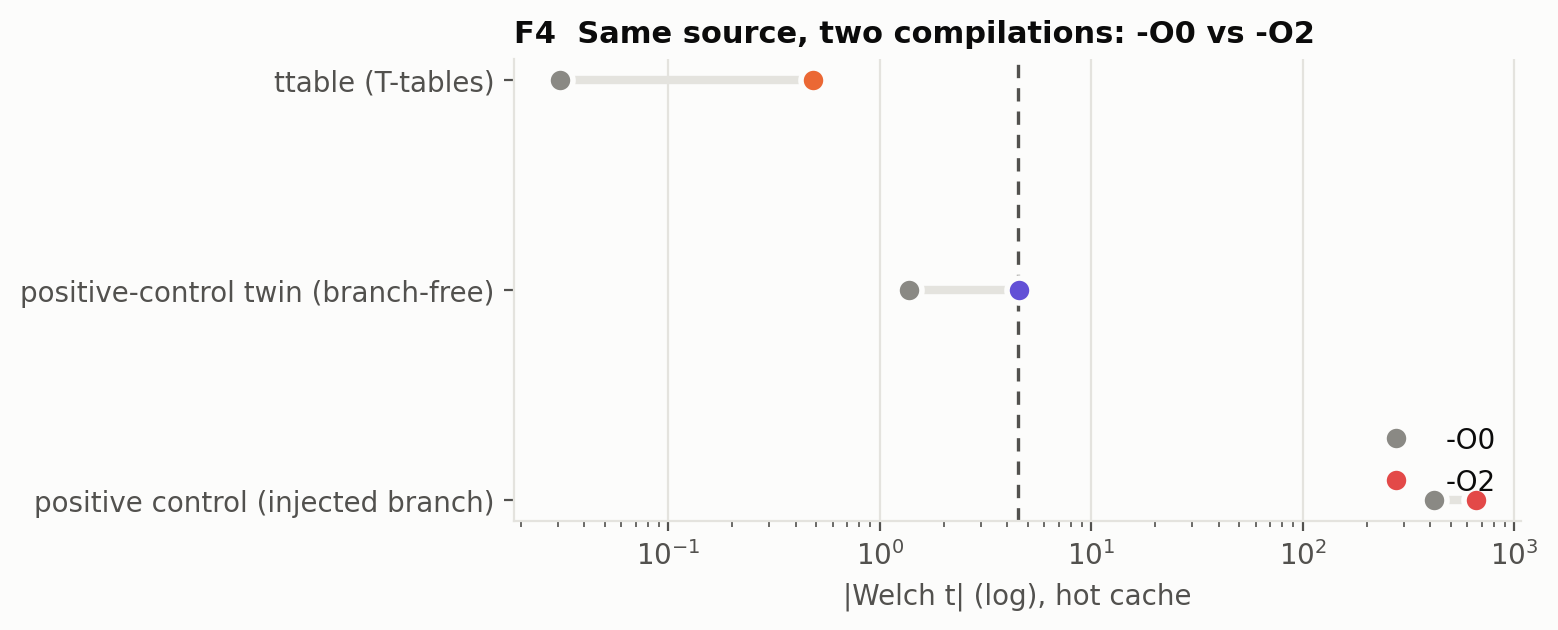
\includegraphics[width=\textwidth]{F4_compiler.png}\\
{\scriptsize \code{-O0} vs.\ \code{-O2}: injected branch detected at both (417, 655)}
\end{column}
\end{columns}
\end{frame}

\begin{frame}{Under the hood: source $\neq$ machine code}
\centering\small
\renewcommand{\arraystretch}{1.15}
\begin{tabular}{@{}ll@{}}
\toprule
& Assembly evidence \\
\midrule
Positive control, \code{-O2} & \code{tbnz w0, \#7} $\rightarrow$ the branch \alert{survives} \\
Twin, \code{-O2} & \code{bic / neg / and / orr}: mask, no branch \\
\code{ttable} & \code{ldr w9, [x14, w9, uxtw \#2]}: \alert{secret address} \\
\code{ct} S-box & 917 instructions, \alert{0 branches, 0 indexed loads} \\
\code{armv8} & 60 \code{aese}, 54 \code{aesmc} \\
OpenSSL default & \code{aes\_v8\_ecb\_encrypt} (hardware) \\
OpenSSL \code{armcap=0} & \code{AES\_encrypt} (portable C, 4.5$\times$ slower) \\
\bottomrule
\end{tabular}
\end{frame}

\begin{frame}{Verdicts, an unexpected result, and limits}
\begin{columns}[T]
\begin{column}{0.44\textwidth}
\small
\renewcommand{\arraystretch}{1.1}
\begin{tabular}{@{}lll@{}}
\toprule
H & Hypothesis & Verdict \\
\midrule
H0 & A/A below 4.5 & \checkmark{} 1.02 \\
H1 & branch detected & \checkmark{} 655 \\
H2 & T-table, evicted & \checkmark{} 18.8 \\
H3 & ct, armv8 quiet & \checkmark{} $\le$1.10 \\
H4 & OpenSSL path & \checkmark{} HW vs C \\
\bottomrule
\end{tabular}
\end{column}
\begin{column}{0.54\textwidth}
\small
\textbf{Unexpected:} branch-free code with a data-dependent load flagged in the \emph{hot, long-batch} regime ($\lvert t\rvert$ 4.5--14); gone at $B \le 10$; mechanism \alert{unexplained} (predictor state? cf.\ SLAP/FLOP)\\[4pt]
\textbf{Limits:} 24 MHz timer \textbullet{} no core pinning on macOS \textbullet{} one machine, one compiler \textbullet{} in-process attacker\\[4pt]
\alert{Detection $\neq$ exploitability; non-detection $\neq$ proof}
\end{column}
\end{columns}
\end{frame}

\partslide{Part II}{ChronoLeak}

\begin{frame}{From Part I to Part II}
\begin{itemize}
  \item Part I lesson: \alert{constant-time is a property of machine code on a CPU}, not of source
  \item Compilers breaking CT code is known for \alert{C} (Breaking Bad, Fun with Flags, DOCC)
  \item Rust has its \alert{own} mechanisms, never measured:
  \begin{itemize}
    \item \code{subtle::Choice}, volatile barrier vs.\ \code{core\_hint\_black\_box}
    \item the \code{Choice} $\rightarrow$ \code{bool} boundary; naive idioms (\code{==} on slices, \code{match})
    \item MIR opts, monomorphisation, codegen-units, LTO, target features, crate backends
  \end{itemize}
\end{itemize}
\vspace{0.2cm}
\begin{block}{Central question}
How do Rust constant-time mechanisms and compiler settings preserve or break secret-independent execution, and when do violations become \emph{measurable}?
\end{block}
\end{frame}

\begin{frame}{Research questions and design}
\begin{columns}[T]
\begin{column}{0.45\textwidth}
\small
\begin{description}[RQ4]
  \item[RQ1] \emph{What}: do barriers survive across rustc/LLVM settings?
  \item[RQ2] \emph{Why}: which stage or pass is responsible?
  \item[RQ3] Which violations are measurable at runtime? \alert{(centre)}
  \item[RQ4] Effect of architecture and load (robustness)
\end{description}
\vspace{0.1cm}
{\scriptsize Targets: \code{subtle}, \code{curve25519-dalek}, \code{k256}, \code{ml-dsa} pre/post fix (positive control)}
\end{column}
\begin{column}{0.53\textwidth}
\centering
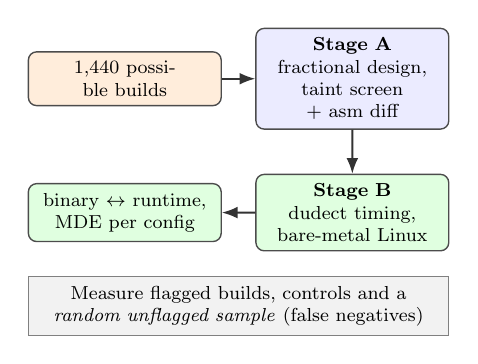
\begin{tikzpicture}[scale=0.85, transform shape]
  \node[impl, text width=2.6cm] (a) at (0,0) {1,440 possible builds};
  \node[sw, text width=2.6cm] (b) at (3.4,0) {\textbf{Stage A}\\ fractional design, taint screen + asm diff};
  \node[res, text width=2.6cm] (c) at (3.4,-2.0) {\textbf{Stage B}\\ dudect timing, bare-metal Linux};
  \node[res, text width=2.6cm] (d) at (0,-2.0) {binary $\leftrightarrow$ runtime, MDE per config};
  \draw[arr] (a) -- (b); \draw[arr] (b) -- (c); \draw[arr] (c) -- (d);
  \node[note, text width=6.0cm] at (1.7,-3.4) {Measure flagged builds, controls and a \emph{random unflagged sample} (false negatives)};
\end{tikzpicture}
\end{column}
\end{columns}
\end{frame}

\begin{frame}{Platforms, software and roadmap}
\begin{columns}[T]
\begin{column}{0.48\textwidth}
\small
\textbf{Platforms}
\begin{itemize}
  \item Linux x86-64 bare metal (primary): \code{rdtscp}, \code{isolcpus}, fixed frequency
  \item Linux AArch64 (Pi 5) second; Apple M4 supplementary
\end{itemize}
\textbf{Tools}: ctgrind-style taint (primary), MicroWalk; Pitchfork time-boxed\\[3pt]
\textbf{Software}: 4 Rust crates (\code{core}, \code{measure}, \code{stats}, \code{cli}) + Python
\end{column}
\begin{column}{0.5\textwidth}
\small
\renewcommand{\arraystretch}{1.08}
\begin{tabular}{@{}ll@{}}
\toprule
Weeks & Milestone \\
\midrule
1--3 & literature, novelty check \\
4--5 & \alert{gate}: Linux box, analyser \\
6--8 & \alert{gate}: \code{subtle} pilot \\
9--12 & ChronoLeak MVP \\
13--19 & screening + timing \\
20--24 & robustness, paper \\
\bottomrule
\end{tabular}

\vspace{0.1cm}
{\scriptsize Pilot outcomes fixed in advance: expand \textbullet{} reframe \textbullet{} stop}
\end{column}
\end{columns}
\end{frame}

\begin{frame}{Conclusions}
\begin{itemize}
  \item Five functionally identical AES-128 implementations behave very differently in time
  \item T-table AES leaks once the cache is flushed; computed S-box and hardware AES show nothing detectable
  \item OpenSSL is safe by default but falls back to a leaky table path if hardware detection is off
  \item \alert{Use hardware AES}: fastest and quietest, but check it is really selected
  \item \alert{Constant-time belongs to machine code on a CPU}: inspect assembly, test with controls, state sensitivity
  \item Part II takes this to Rust: do the language's constant-time mechanisms survive the compiler?
\end{itemize}
\vspace{0.2cm}
{\small Future work: cycle counters \textbullet{} DIT on whole implementations \textbullet{} Prime+Probe \textbullet{} bit-sliced AES \textbullet{} ChronoLeak pilot}
\end{frame}

\begin{frame}{References and tools}
\tiny
\begin{itemize}
  \item NIST FIPS 197 (AES), SP 800-38A \textbullet{} Daemen \& Rijmen, \emph{The Design of Rijndael}, 2002
  \item Kocher, CRYPTO 1996 \textbullet{} Bernstein, \emph{Cache-timing attacks on AES}, 2005 \textbullet{} Osvik, Shamir \& Tromer, CT-RSA 2006
  \item Goodwill et al., TVLA, NIAT 2011 \textbullet{} Reparaz et al., dudect, DATE 2017 \textbullet{} Welch, \emph{Biometrika} 1947
  \item Käsper \& Schwabe, CHES 2009 \textbullet{} Hamburg, CHES 2009
  \item Chen et al., GoFetch, USENIX Sec 2024 \textbullet{} Kim et al., FLOP, USENIX Sec 2025 \textbullet{} Kim et al., SLAP, IEEE S\&P 2025
  \item Schneider et al., Breaking Bad, ASIA CCS 2025 \textbullet{} Geimer \& Maurice, Fun with Flags, PriSC 2026 \textbullet{} Gerlach et al., DOCC, FC 2025
  \item Kolosick et al., RoboCop, PLDI 2025 \textbullet{} Wichelmann et al., MicroWalk, ACSAC 2018 \textbullet{} Lai et al., AutoBench-CT, ePrint 2026/2682
  \item ctgrind \textbullet{} haybale-pitchfork \textbullet{} dudect-bencher \textbullet{} \code{subtle} \textbullet{} \code{core::hint::black\_box}
  \item RUSTSEC-2025-0144 \textbullet{} CVE-2025-12888 \textbullet{} Trail of Bits, LLVM \code{ct.select} (2025)
\end{itemize}
\vspace{0.2cm}
\scriptsize
\textbf{Libraries:} OpenSSL 3.6.1, Chart.js 4.4.7, NumPy, SciPy, pandas, Matplotlib, CMake, Apple Clang 21, Tectonic/Beamer\\
\textbf{AI tools:} ChatGPT (OpenAI), used for [Bibek: what it was used for]\\
\textbf{Code, report and data:} \code{github.com/bibek198/AES-Under-the-Microscope}, recorded run \code{full-20261117-0301}
\end{frame}

{\setbeamercolor{background canvas}{bg=ink}\setbeamertemplate{footline}{}
\begin{frame}[plain]
\centering\color{white}\vfill
{\Huge\bfseries Thank you}\par\vspace{0.3cm}
{\large Questions?}\par\vfill
\end{frame}}

\end{document}
